% Тип документа
\documentclass[a4paper,14pt]{extarticle}

% Шрифты, кодировки, символьные таблицы, переносы
\usepackage{cmap}
\usepackage[T2A]{fontenc}
\usepackage[utf8x]{inputenc}
\usepackage[russian]{babel}
\usepackage[table]{xcolor}
% Это пакет -- хитрый пакет, он нужен но не нужен
\usepackage[mode=buildnew]{standalone}

\usepackage
	{
		% Дополнения Американского математического общества (AMS)
		amssymb,
		amsfonts,
		amsmath,
		amsthm,
		physics,
		% misccorr,
		% 
		% Графики и рисунки
		wrapfig,
		graphicx,
		subcaption,
		float,
		tikz,
		tikz-3dplot,
		caption,
		csvsimple,
		color,
		booktabs,
		pgfplots,
		pgfplotstable,
		geometry,
		% 
		% Таблицы, списки
		array,
		makecell,
		multirow,
		indentfirst,
		%
		% Интегралы и прочие обозначения
		ulem,
		esint,
		esdiff,
		% 
		% Колонтитулы
		fancyhdr,
	}  

\usepackage{xcolor}
\usepackage{hyperref}

 % Цвета для гиперссылок
\definecolor{linkcolor}{HTML}{000000} % цвет ссылок
\definecolor{urlcolor}{HTML}{799B03} % цвет гиперссылок
 
\hypersetup{pdfstartview=FitH,  linkcolor=linkcolor,urlcolor=urlcolor, colorlinks=true}
% Обводка текста в TikZ
\usepackage[outline]{contour}

% Увеличенный межстрочный интервал, французские пробелы
\linespread{1.1} 
\frenchspacing 

 
\usetikzlibrary
	{
		decorations.pathreplacing,
		decorations.pathmorphing,
		patterns,
		calc,
		scopes,
		arrows,
		fadings,
		through,
		shapes.misc,
		arrows.meta,
		3d,
		quotes,
		angles,
		babel
	}

\usepgfplotslibrary{units}

% const прямым шрифтом
\newcommand\ct[1]{\text{\rmfamily\upshape #1}}
\newcommand*{\const}{\ct{const}}
\renewcommand*{\epsilon}{\varepsilon}

\usepackage[europeanresistors,americaninductors]{circuitikz}

% Style to select only points from #1 to #2 (inclusive)
\pgfplotsset{select/.style 2 args={
    x filter/.code={
        \ifnum\coordindex<#1\def\pgfmathresult{}\fi
        \ifnum\coordindex>#2\def\pgfmathresult{}\fi
    }
}}

\usepackage{array}
\usepackage{pstool}

%%%%%%%%%%%%%%%%%%%%%%%%%%%%%%%%%%%%%%%%%%%%%%%%%
\makeatletter
\newif\if@gather@prefix 
\preto\place@tag@gather{% 
  \if@gather@prefix\iftagsleft@ 
    \kern-\gdisplaywidth@ 
    \rlap{\gather@prefix}% 
    \kern\gdisplaywidth@ 
  \fi\fi 
} 
\appto\place@tag@gather{% 
  \if@gather@prefix\iftagsleft@\else 
    \kern-\displaywidth 
    \rlap{\gather@prefix}% 
    \kern\displaywidth 
  \fi\fi 
  \global\@gather@prefixfalse 
} 
\preto\place@tag{% 
  \if@gather@prefix\iftagsleft@ 
    \kern-\gdisplaywidth@ 
    \rlap{\gather@prefix}% 
    \kern\displaywidth@ 
  \fi\fi 
} 
\appto\place@tag{% 
  \if@gather@prefix\iftagsleft@\else 
    \kern-\displaywidth 
    \rlap{\gather@prefix}% 
    \kern\displaywidth 
  \fi\fi 
  \global\@gather@prefixfalse 
} 
\newcommand*{\beforetext}[1]{% 
  \ifmeasuring@\else
  \gdef\gather@prefix{#1}% 
  \global\@gather@prefixtrue 
  \fi
} 
\makeatother
%%%%%%%%%%%%%%%%%%%%%%%%%%%%%%%%%%%%%%%%%%%%%%%%%

\geometry		
	{
		left			=	2cm,
		right 			=	2cm,
		top 			=	3cm,
		bottom 			=	3cm,
		bindingoffset	=	0cm
	}

%%%%%%%%%%%%%%%%%%%%%%%%%%%%%%%%%%%%%%%%%%%%%%%%%%%%%%%%%%%%%%%%%%%%%%%%%%%%%%%

	%применим колонтитул к стилю страницы
\pagestyle{fancy} 
	%очистим "шапку" страницы
\fancyhead{} 
	%слева сверху на четных и справа на нечетных
\fancyhead[R]{\labauthors} 
	%справа сверху на четных и слева на нечетных
\fancyhead[L]{Отчёт по лабораторной работе №\labnumber} 
	%очистим "подвал" страницы
\fancyfoot{} 
	% номер страницы в нижнем колинтуле в центре
\fancyfoot[C]{\thepage} 

%%%%%%%%%%%%%%%%%%%%%%%%%%%%%%%%%%%%%%%%%%%%%%%%%%%%%%%%%%%%%%%%%%%%%%%%%%%%%%%

\renewcommand{\contentsname}{Оглавление}

\usepackage{tocloft}
% \renewcommand{\cftpartleader}{\cftdotfill{\cftdotsep}} % for parts
% \renewcommand{\cftsectiondotsep}{\cftdotsep}% Chapters should use dots in ToC
\renewcommand{\cftsecleader}{\cftdotfill{\cftdotsep}}
%\renewcommand{\cftsecleader}{\cftdotfill{\cftdotsep}} % for sections, if you really want! (It is default in report and book class (So you may not need it).
% ---------
% \newcommand{\cftchapaftersnum}{.}%
% \usepackage{titlesec}
% \titlelabel{\thetitle.\quad}
\usepackage{secdot}
\sectiondot{subsection}
\newcommand{\rot}{\operatorname{rot}}

\begin{document}

\def\labauthors{Карусевич А.А., Шиков А.П.}
\def\labgroup{440}
\def\labnumber{1}
\def\labtheme{Волноводные ферритовые устройства СВЧ диапазона}
\begin{titlepage}

\begin{center}

{\small\textsc{Нижегородский государственный университет имени Н.\,И. Лобачевского}}
\vskip 1pt \hrule \vskip 3pt
{\small\textsc{Радиофизический факультет. Кафедра Электродинамики.}}

\vfill

{\Large Отчет по лабораторной работе №\labnumber\vskip 12pt\bfseries \labtheme}
	
\end{center}

\vfill
	
\begin{flushright}
	{Выполнили студенты \labgroup\ группы\\ \labauthors}%\vskip 12pt Принял:\\ Менсов С.\,Н.}
\end{flushright}
	
\vfill
	
\begin{center}
	Нижний Новгород, \the\year
\end{center}

\end{titlepage}



\newpage

{\bfseries Цель работы:} 
Изучение электродинамических систем, содержащих гиротропные элементы - ферриты.

\section{Теоритическая часть}
\subsection{Введение}
Известно, что в линейных анизотропных средах с симметричными тензорами диэлектрической и магнитной проницаемости
$\epsilon_{ij} = \epsilon_{ji},\mu_{ij} = \mu_{ji}$ (а также в обычных изотропных средах) имеет место теорема взаимности. Эта теорема оказывается несправедливой в средах
с несимметричными тензорами проницаемостей, в частности, в так называемых гиротропных средах, к которым принадлежат
плазма и ферриты, находящиеся во внешнем постоянном магнитном ноле.

Используя невзаимные свойства гиротропных сред, можно создавать устройства, канализирующие электромагнитные волны в
одном направлении и почти не пропускающие в противоположном направлении. Этим объясняется широкое применение ферритов в
волноводных устройствах сверхвысоко-частотного (СВЧ) диапазона. К настоящему времени разработано большое количество
устройств с ферритовыми элементами, имеющих различные конструктивные исполнения и электродинамические характеристики.

\subsection{Анизотропные и гиротропные среды}

Анизотропными средами называются среды, локальные макроскопические свойства которых различны в различных направлениях.
Анизотропией обладают многие жидкости и большинство кристаллов. Поликристалличе-ские вещества становятся анизотропными
под воздействием давления, статических электрических и магнитных полей. Наряду с анизотропными существуют среды,
локальные макроскопические свойства которых поиштрнапт-ны относительно зеркальных отражений, т.е. изменяются при
некоторых зеркальных отражениях. Такие среды называются оетостноппонктшшыми (пли гиротропными). Примерами таких сред
могут служить кристаллы без центра симметрии или среды, состоящие из частиц, не обладающих центром симметрии. Некоторые
среды приобретают гиротропные свойства при наложении внешнего магнитного поля. Такие среды принято называть
магнито-активными. Типичными примерами магиитоактивиых сред являются плазма и ферриты, находящиеся во внешнем постоянном
магнитном поле.

\textit{Ферриты}, представляют собой химические соединения оксида железа с оксидами других, так называемых характеризующих
металлов (никеля, кобальта, магния, марганца, кадмия и т. д.). Особенностью этих материалов является сочетание
гиротропных свойств с низкой электропроводностью, благодаря чему электромагнитные волны при определенных условиях могут
распространяться в ферритах с достаточно малым затуханием.

Магнитные свойства ферритов определяются наличием в их кристаллической решетке атомов или ионов, обладающих отличным от
нуля магнитным моментом. В отсутствие внешнего магнитного поля магнитные моменты ориентированы хаотически, и в целом
феррит изотропен. В достаточно сильном постоянном магнитном поле $\textbf{H}_0$ магнитные моменты всех атомов за время
$\tau_0 \simeq (10^{-9} - 10^{-7})$ с (время релаксации) устанавливаются по направлению магнитного поля. В этом состоянии феррит обладает
значительной намагниченностью и становится анизотропной гиротроппой средой по отношению к высокочастотному электромагнитному полю.

В линейном анизотропном магнетике каждая компонента вектора магнитной индукции $\textbf{B}$ представляет собой линейную функцию
трех компонент ноля $\textbf{H}$:
\begin{equation}
    \begin{aligned} 
        B_{x} &=\mu_{x x} H_{x}+\mu_{x y} H_{y}+\mu_{x z} H_{z} \\
        B_{y} &=\mu_{y x} H_{x}+\mu_{y y} H_{y}+\mu_{y z} H_{z} \\
        B_{z} &=\mu_{z x} H_{x}+\mu_{z y} H_{y}+\mu_{z z} H_{z}
    \end{aligned}
    \label{eq:1}
\end{equation}
Величины $\mu_{i j}(i,j=x,y,z)$, входящие в соотношения \eqref{eq:1}, являются компонентами тензора второго ранга, называемого
тензором магнитной проницаемости:
\begin{equation}
    \hat{\mu}=\left(\begin{array}
        {ccc}{\mu_{x x}} & {\mu_{x y}} & {\mu_{x z}} \\
        {\mu_{y x}} & {\mu_{y y}} & {\mu_{y z}} \\
        {\mu_{z x}} & {\mu_{z y}} & {\mu_{z z}}
    \end{array}\right)
    \label{eq:2}
\end{equation}


С учетом \eqref{eq:2} материальные уравнения \eqref{eq:1} можно записать в удобной матричной форме

\begin{equation}
    \textbf{B} = \hat{\mu}\textbf{H}
    \label{eq:3}
\end{equation}

При наличии в феррите электромагнитного поля, изменяющегося во времени но гармоническому закону и имеющего напряженность
$\textbf{H}(\textbf{r})e^{i\omega t}$, малую но сравнению с постоянным магнитным полем $\textbf{H}_0 =
H_0\textbf{z}_0(|\textbf{H}|\ll H_0)$, тензор магнитной проницаемости $\hat{\mu}$ принимает вид

\begin{equation}
    \hat{\mu}=\left(\begin{array}
        {ccc}{\mu} & {i\mu_{a}} & {0} \\
        {-i\mu_{a}} & {\mu} & {0} \\
        {0} & {0} & {\mu_{||}}
    \end{array}\right)
    \label{eq:4}
\end{equation}

\begin{equation}
    \mu=1+\frac{4 \pi \chi \omega_{H}^{2}}{\omega_{H}^{2}-\omega^{2}}, 
    \quad \mu_{a}=\frac{4 \pi \chi \omega_{H} \omega}{\omega_{H}^{2}-\omega^{2}}, 
    \quad \mu_{ \|}=1
    \label{eq:5}
\end{equation}
Здесь $\omega$ - круговая частота, $\chi$ - статическая магнитная восприимчивость феррита, $\omega_H = \frac{e H_0}{m
c}$ - гирочастота электрона ($m$ и $e$ — масса и абсолютное значение заряда электрона соответственно, $c$ — скорость света в вакууме).


Обратим внимание на то, что тензор \eqref{eq:4} подчиняется соотношению $\mu_{ij} = \mu_{ji}^*$ т. е. является эрмитовым (знак «*» означает
операцию комплексного сопряжения). Данное свойство имеет место для сред при пренебрежении потерями.

В отсутствие статического магнитного поля $(\textbf{H}_0 = 0)$ недиагональные элементы тензора \eqref{eq:4} обращаются в пуль, диагональные
компоненты $\mu$ и $\mu_{||}$ принимают одинаковые значения ($\mu=\mu_{||}$), и феррит становится изотропным.

При стремлении частоты поля $\omega$ к гирочастоте $\omega_H$ компоненты $\mu$ и $\mu_a$ обращаются в бесконечность. Это явление называют
ферромагнитным резонансом. В действительности из-за диссипативных процессов элементы тензора $\mu$ и $\mu_a$ становятся весьма
большими, но не бесконечными. Потери в феррите в случае малой диссипации можно учесть феноменологически , заменив
частоту $\omega_H$ в выражениях \eqref{eq:5} па комплексную величину $\tilde{\omega}_H = \omega_H+ i \gamma \omega$, где
$\gamma$ — безразмерный параметр диссипации ($\gamma \ll 1$).

\begin{figure}[h!]
    \centering
    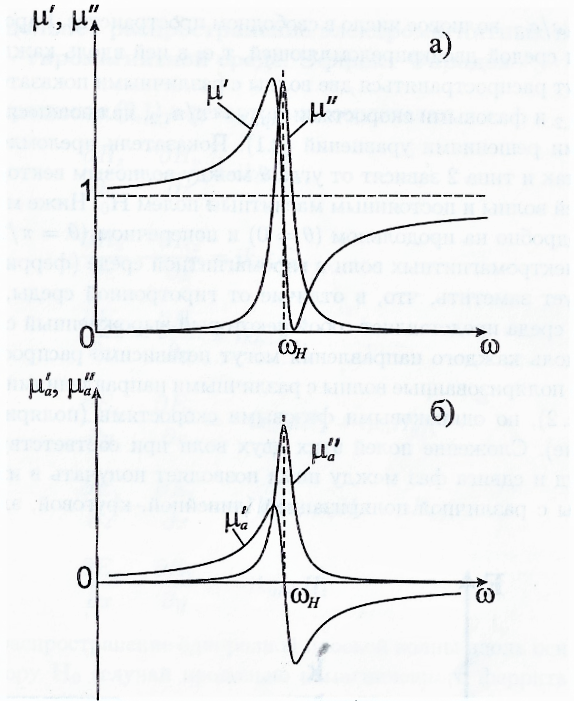
\includegraphics[width = 0.5\linewidth]{imgs/temp/001.png}
    \caption{Качественный вид зависимостей величин $\mu^{\prime}$, $\mu^{\prime \prime}(a)$ и 
    $\mu_{a}^{\prime}$, $\mu_{a}^{\prime \prime}$(b) от частоты $\omega$}
    \label{fig:1}
\end{figure}

Таким образом, при учете потерь величины $\mu$ и $\mu_{a}$ являются комплексными, т. е. $\mu=\mu^{\prime}-i \mu^{\prime \prime}, 
\mu_{a}=\mu_{a}^{\prime}-i \mu_{a}^{\prime \prime}$, а тензор $\hat{\mu}$ перестает быть эрмитовым ($\mu_{ij} \neq
\mu_{ji}^*$). Качественные зависимости действительных и мнимых частей этих величин от частоты
$\omega$ при фиксированном статическом поле $H_0$ показаны на рис. 1. Из рис. 1 видно, что в случае $\omega=\omega_H$ и
величины $\mu^{\prime \prime}$ и $\mu_{a}^{\prime \prime}$ максимальны, что свидетельствует о резонансном поглощении
электромагнитного поля ферритом. Следует отметить, что в ограниченных ферритовых образцах внутреннее статическое
магнитное поле $\textbf{H}_0$ отличается от внешнего поля $\textbf{H}_{\text{ВН}}$, в которое
помещен образец. Поэтому частота ферромагнитного резонанса при заданном поле $\textbf{H}_{\text{ВН}}$ зависит от формы образца и его
ориентации относительно внешнего магнитного поля. Для определения внутреннего ноля в образце следует решить
соответствующую краевую задачу магнитостатики.

\subsection{Распространение электромагнитных волн в гиротропной среде}
\subsubsection{Продольное распространение электромагнитных волн в гиромагнитной среде. Эффект Фарадея}
\subsubsection{Поперечное распространение электромагнитных волн в гиромагнитной среде}
\subsection{Волновод, слабо заполненный ферритом}
\subsection{Рассчет постоянных распространения собственных мод в волноводе, слабо заполненном ферритом}

\newpage
\section{Экспериментальная часть}

% Схема установки:
% \begin{figure}[H]
%     \centering
%     \includegraphics[width = 0.7\linewidth]{imgs/exp.png}
% \end{figure}
Оборудование: 
\begin{itemize}
    \item Генератор СВЧ излучения с регулируемыми частотой и ослаблением.
    \item Волноводный переключатель с взаимным фазовращателем
    \item Циркулятор на эффекте Фарадея
    \item Волноводный вентиль
    \item Измерительный тракт
    \item Согласованные нагрузки
\end{itemize}
Во всех экспериментах частота генератора $f_g$ была постоянной и не изменялась: $f_g = 10.6$ ГГц.
\subsection{Волноводный переключатель}
Взаимный фазовращатель представляет собой отрезок прямоугольного волновода с продольно намагниченным ферритом,
расположенным вдоль центральной оси волновода. Путем изменения поля подмагничивания фазовращатель
позволяет регулировать набег фазы на участке волновода с ферритом. Два таких фазовращателя используются в волноводном
переключателе, изображенном схематически на рис. \ref{fig:ex:1}. В переключателе мощность высокочастотных электромагнитных колебаний,
поступающих из генератора, делится поровну между двумя волноводными секциями, в которых помещены одинаковые ферритовые
стержни, подмагничиваемые с помощью соленоидов. Размеры секций подобраны таким образом, что в каждой из них (при
используемой частоте генератора) распространяющейся является только волна низшего типа $TE_{10}$. Затем высокочастотная
мощность поступает в волноводно-щелевой мост, па выходе которого перераспределяется между двумя волноводами.

\begin{figure}[h!]
    \centering
    \includegraphics[width = 0.5\linewidth]{example-image-a}
    \caption{Волноводный переключатель с взаимным фазовращателем}
    \label{fig:ex:1}
\end{figure}

Волноводно-щелевой мост сконструирован таким образом, что мощность, поступающая в любое из его плеч (1 или 2), поровну
распределяется между противоположными плечами (3 или 4), причем фаза волны в дальнем плече отстает от фазы волны в
ближнем плече на $\pi/2$. Мост имеет вид сдвоенных прямоугольных волноводов, в общей широкой стенке которых прорезана одна
или несколько щелей. В лабораторной установке щели прорезаны от одной узкой стенки до другой, а размеры $a_1=a$ и $b_1$
поперечного сечения области, образованной сдвоенными волноводами (область связи), выбраны такими, чтобы в пей могли
распространяться волны только трех типов $TE_{10}$, $TE_{01}$, $TE_{11}$.

Работу волноводно-щелевого моста удобно пояснить с помощью векторных диаграмм (рис. \ref{fig:ex:2}). На таких диаграммах поле в
соответствующем плече моста изображается вектором, длина которого равна абсолютному значению поля, а угол поворота
относительно направления $\phi = 0$ — фазе поля. 
\begin{figure}[h!]
    \centering
    \includegraphics[width = 0.8\linewidth]{example-image-b}
    \caption{Векторные диаграммы, поясняющие работу волноводно-щелевого моста}
    \label{fig:ex:2}
\end{figure}
\subsection{Циркулятор на эффекте Фарадея}
\subsection{Волноводный вентиль}

\subsection{Вывод}

\newpage
\section{Приложение}

\end{document}